% Point avec Caroline Hillairet (tutrice de stage), 10 aout 2026. DIX slides pour QUINZE
% minutes, dont une de RESERVE (la derniere) et une de figure seule.
%
% VERSION REECRITE SUR DEMANDE DE KELIAN, ET LE PERIMETRE A CHANGE. Deux consignes explicites :
%   1. NE PAS CITER LE MEMOIRE. On parle du MODELE et de son avancement, jamais du document :
%      pas de compte de pages, pas de taux de harnais, pas de numero de chapitre. Ce sont des
%      metadonnees de redaction, sans interet pour une tutrice de stage.
%   2. NE PAS PARLER DU PROCESSUS DE HAWKES. La section C de la version precedente et sa slide
%      de figure ont donc ete RETIREES, avec la figure O2 qui les portait.
%
% CONSEQUENCE PRATIQUE A CONNAITRE : la sortie non versionnee du script 08h ne bloque plus ce
% point, puisque plus aucun chiffre du deck n'en depend. Elle reste a produire pour le suivi
% interne, mais elle sort du chemin critique de ce call.
%
% CE QUE LE DECK FAIT DESORMAIS, DANS L'ORDRE : expliquer la modelisation retenue (slides 3 a 5),
% rendre compte du dernier point tuteur du 07/08 (slide 6), puis poser les demandes d'appui
% (slides 7 et 8). La slide 9 est une reserve, a sacrifier sans regret.
%
% CE QUI L'ENGAGE PERSONNELLEMENT, ET C'EST CE QUI OUVRE LA PARTIE DEMANDES :
%   1. Sa remarque « le quantile d'un objet incertain est mauvais » a produit deux briques du
%      modele, la VaR predictive (script 46) et la bande de modele (script 48). Slide 7.
%   2. Le modele emprunte a Hillairet et Lopez la logique d'etats de conformite.
%
% BUDGET DE TEMPS SUR 15 MIN : ouverture 1 ; modelisation 3 ; schema 2 ; cascade 3 ; point
% tuteur 2 ; postures et question 3 ; trois questions 1. La slide a ne jamais presser est la 7 :
% c'est la seule qui appelle une DECISION de sa part.
%
% FIGURE. Une seule, schema_modele.pdf, JAMAIS utilisee dans un deck precedent (verifie sur les
% huit fichiers de exploratory/slides/). Elle est en A4 PAYSAGE, ratio 0,71, donc contrainte en
% HAUTEUR et seule sur sa slide : posee en largeur elle ferait 76 mm pour 74 mm utiles. Son
% interet ici est que chaque grandeur y porte une pastille de STATUT (estimee, posee, bornee,
% reglementaire), ce qui permet d'attaquer le modele bloc par bloc.
\documentclass[11pt]{beamer}
\usetheme{Madrid}
\usecolortheme{seahorse}
\usepackage[utf8]{inputenc}
\usepackage[T1]{fontenc}
\usepackage[french]{babel}
\usepackage{booktabs}
\usepackage{amsmath,amssymb}
\usepackage{eurosym}
\graphicspath{{../vasicek_lab/figures/}{../vasicek_lab/notes/}}
\setbeamertemplate{navigation symbols}{}
\setbeamertemplate{caption}{\raggedright\insertcaption\par}
\setbeamerfont{block title}{size=\small}

\title[Point de stage]{Quantification du risque de non-conformité DORA}
\subtitle{La modélisation retenue, le dernier point tuteur, et quatre demandes d'appui}
\author[K. Kaddouri]{Kélian Kaddouri}
\institute[ENSAE / Nexialog]{ENSAE / Nexialog Consulting}
\date[10/08/2026]{10 août 2026}

\begin{document}

% HARNAIS-HORS-SECTION: page de titre et slide de sommaire, avant la premiere \section*. Les
%   nombres y sont la date, la duree du point et la numerotation des trois temps : aucun
%   resultat de modele, donc rien qu'un script doive produire. Le motif decrit bien la PORTEE
%   de la declaration, qui couvre DEUX frames et non la seule page de titre : une declaration
%   dont le motif est plus etroit que sa portee est une exemption silencieuse.

\begin{frame}
\titlepage
\end{frame}

% =====================================================================
\begin{frame}{Le fil de ce point}
\small
Quinze minutes, trois temps. Je passe l'essentiel du temps sur le troisième.
\vspace{2mm}
\begin{block}{Ce que je voudrais couvrir}
\textbf{1. La modélisation retenue à ce jour}, en trois briques et une difficulté centrale.
C'est court, mais nécessaire pour que les questions qui suivent aient un sens.\\[3pt]
\textbf{2. Ce que le point avec mon tuteur du 7 août a produit}, dont deux corrections de fond
qui touchent au vocabulaire et au statut de ce que je publie.\\[3pt]
\textbf{3. Quatre demandes d'appui}, toutes sur la modélisation. La première appelle un
arbitrage qui ne relève pas du calcul, et c'est celle sur laquelle je voudrais m'attarder.
\end{block}
\vspace{1mm}
{\footnotesize Une seule des quatre demandes exige une décision. Les trois autres sont des
questions de méthode sur lesquelles je suis bloqué ou incertain.}
\end{frame}

% =====================================================================
\section*{1. La modélisation}

\begin{frame}{Trois briques, et ce que chacune apporte}
\scriptsize
L'objet est de quantifier un besoin de capital associé à un défaut de maîtrise du risque
informatique, en traitant les cinq domaines d'exigences du règlement DORA comme des composantes
qui se propagent l'une sur l'autre, et non comme des risques indépendants à agréger.
\vspace{1.5mm}
\begin{block}{La fréquence}
Binomiale négative pilotée par un facteur systémique commun, calibrée à $21{,}56$ incidents
informatiques matériels par an à l'échelle du secteur financier mondial. Pour descendre à une
entité, la fréquence n'est pas prise dans une tranche de la base mais \textbf{lue sur une
courbe} : elle est estimée comme une fonction de la taille de firme, log-actifs en covariable,
l'élasticité valant $0{,}0744$.
\end{block}
\vspace{-1mm}
\begin{block}{La sévérité}
Dépassements de seuil et ajustement de Pareto généralisée au-delà de $u = 20{,}03$~M\euro, sur
$91$ excès : $\hat\xi = 0{,}5954$, $\hat\sigma = 57{,}97$. Cette valeur est en elle-même une
information : \textbf{au-dessus de $0{,}5$ la variance est infinie, en dessous de $1$ l'espérance
existe encore}. Le quantile extrême est donc porté par un sinistre unique et non par une
accumulation, ce qui conditionne tout ce qui suit.
\end{block}
\vspace{1mm}
\textbf{L'agrégation}, où se situe l'apport : la propagation est modélisée explicitement plutôt
que les marges couplées par une copule. J'y viens dans deux slides.
\vspace{-0.5mm}

{\scriptsize Sources : scripts~\texttt{07}, \texttt{47}, \texttt{60} et~\texttt{63}.}
\end{frame}

% =====================================================================
% LA FIGURE A SA PROPRE SLIDE, ET ELLE EST CONTRAINTE EN HAUTEUR. Voir l'en-tete : A4 paysage,
% ratio 0,71, elle ne tient pas en largeur dans un cadre qui porte aussi du texte.
\begin{frame}{Le modèle en un schéma, et le statut de chaque grandeur}
\begin{center}
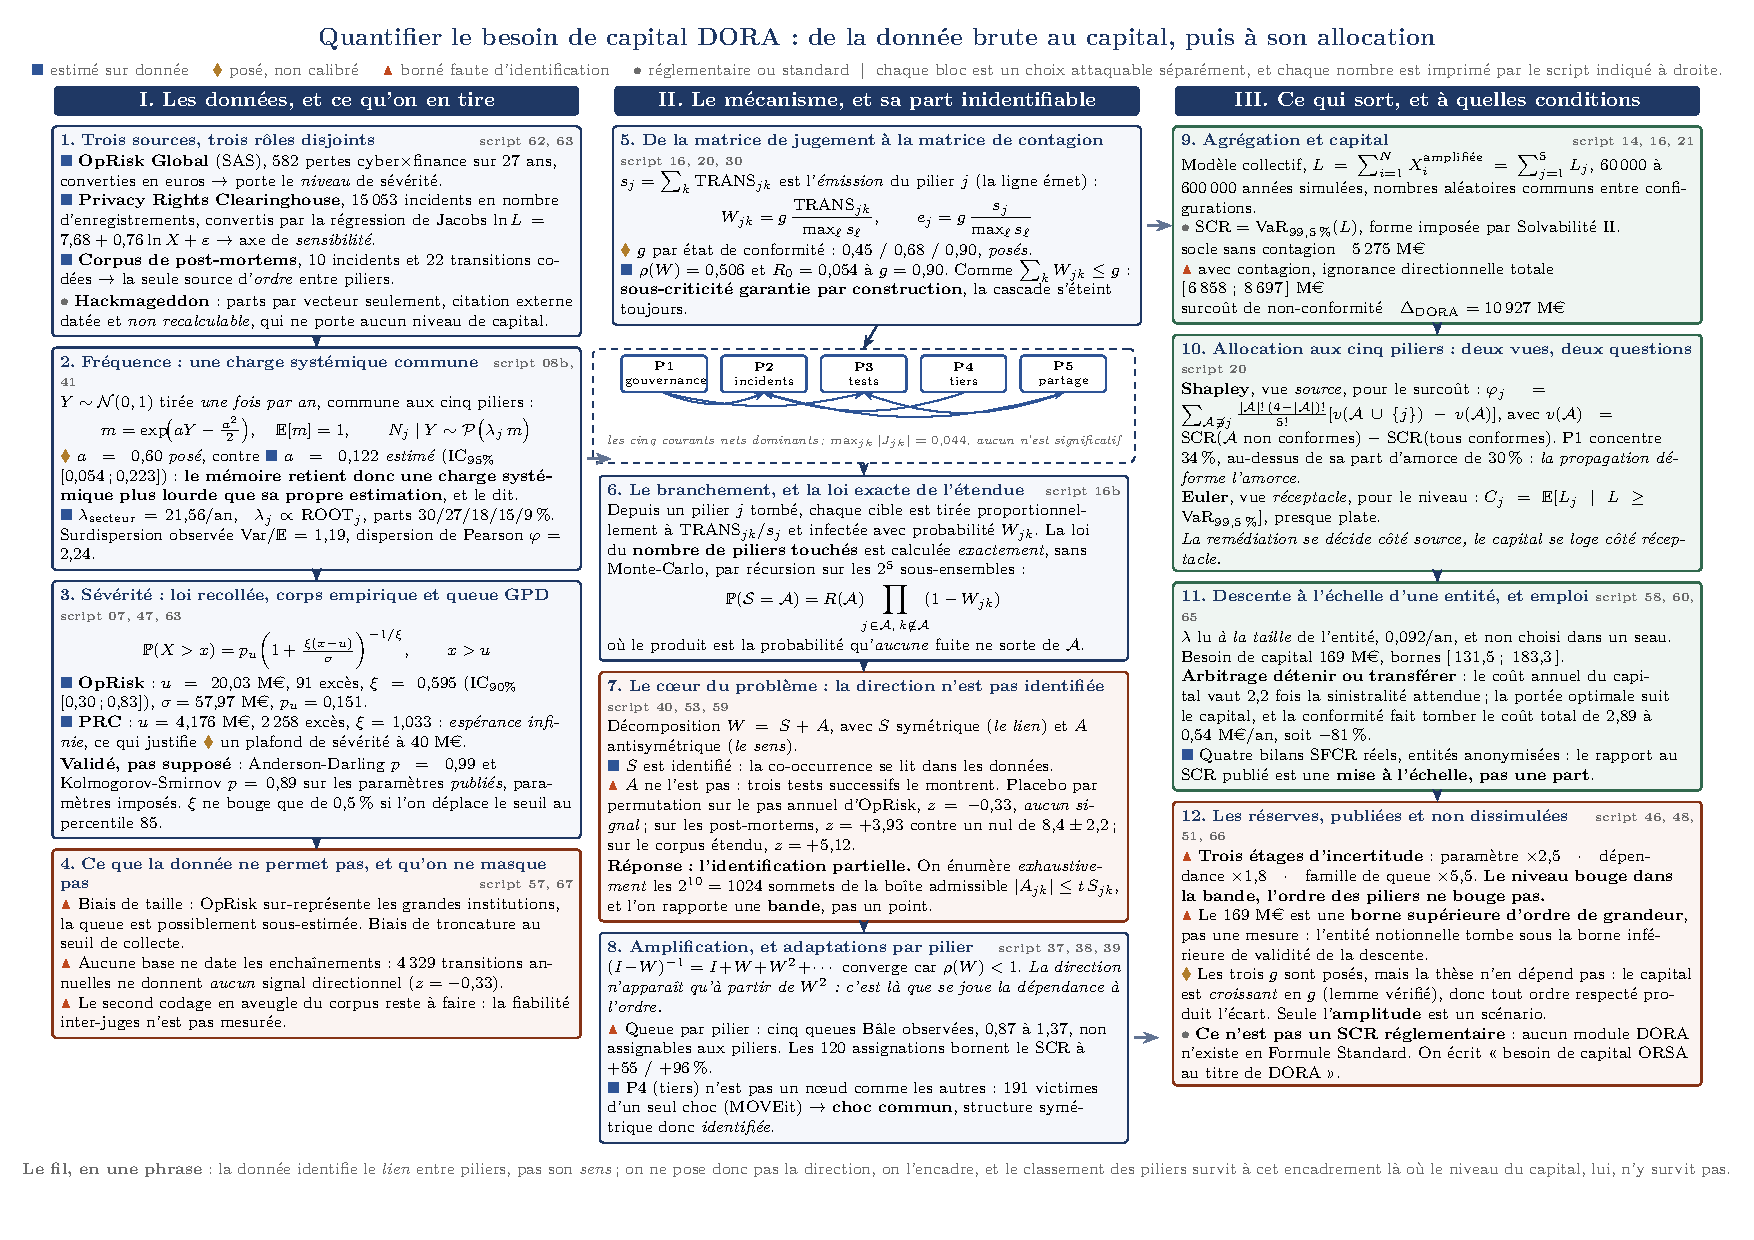
\includegraphics[height=0.72\textheight]{schema_modele.pdf}
\end{center}
{\scriptsize Chaque grandeur porte une pastille de statut : \textbf{estimée}, \textbf{posée},
\textbf{bornée} faute d'identification, ou \textbf{réglementaire}, pour qu'on puisse attaquer le
modèle bloc par bloc.}
\end{frame}

% =====================================================================
\begin{frame}{La propagation, et pourquoi je publie une bande et non un point}
\scriptsize
\begin{block}{Le mécanisme}
Une matrice de propagation va du domaine \textbf{source} vers le domaine \textbf{cible},
normalisée pour que le domaine le plus prolifique engendre au plus $g$ descendants directs. Rayon
spectral $0{,}506$, donc cascade \textbf{sous-critique}, et nombre de reproduction $0{,}054$ :
ce n'est pas un régime épidémique, c'est un amplificateur borné.
\end{block}
\vspace{-1mm}
\begin{block}{La difficulté centrale, et le choix qu'elle impose}
Les bases d'incidents identifient la \textbf{co-occurrence} de deux domaines défaillants, pas
l'ordre dans lequel ils ont cédé : en décomposant la matrice en parties symétrique et
antisymétrique, la donnée identifie la première et \textbf{pas la seconde}, qui est la
direction.\\[3pt]
Je ne tranche donc pas arbitrairement : j'énumère les $2^{10} = 1\,024$ sommets de l'ensemble
admissible et je publie l'\textbf{ensemble} des valeurs compatibles. Socle sans propagation
$5\,275$~M\euro, bornes $[6\,858\,;8\,697]$. Je peux dire que la propagation ajoute au socle, et
de combien au plus et au moins, sans prétendre savoir de combien exactement.
\end{block}
\vspace{-1mm}
{\scriptsize J'avais posé au départ une propriété de \textbf{non-transitivité} de la
propagation : je l'ai testée et réfutée moi-même, et elle est remplacée par une
\textbf{dépendance à l'ordre}, plus faible et qui tient.
\ Sources : scripts~\texttt{03}, \texttt{30} et~\texttt{31}.}
\end{frame}

% =====================================================================
\section*{2. Le dernier point tuteur}

\begin{frame}{Ce que le point du 7 août a produit}
\scriptsize
Trois choses, dont deux corrections de fond.
\vspace{1.5mm}
\begin{block}{Une confusion d'échelles, levée}
Je présentais sous la même étiquette un quantile de \textbf{sévérité}, sur un sinistre unique, et
un besoin de capital, sur la \textbf{charge annuelle agrégée} : cela fait lire une différence
d'échelle comme une incohérence, et la séance a buté là. Le vocabulaire est séparé et le passage
d'une échelle à l'autre est calculé. Ce qui ferme la question : le rapport entre les deux
\textbf{s'inverse selon l'échelle}, donc aucun rapport fixe ne les relie.
\end{block}
\vspace{-1mm}
\begin{block}{Le statut de la mesure de queue, précisé}
Faut-il fonder le capital sur une espérance conditionnelle de queue plutôt que sur un quantile ?
L'argument qui tranche n'est pas le degré de prudence mais l'\textbf{existence} : sur ma seconde
source de sévérité, $\hat\xi = 1{,}033 > 1$, donc \textbf{la mesure n'est pas définie}. Je
l'utilise en diagnostic, jamais en couverture.
\end{block}
\vspace{-1mm}
\begin{block}{Une comparaison retirée, et la calibration gelée}
Je rapportais mon résultat à la charge forfaitaire de Formule Standard. J'ai retiré cette
comparaison : le rapport varie d'un facteur cinquante selon la composition du bilan, donc son
\emph{niveau} ne mesure rien. Reste que le forfait est \textbf{identique quel que soit l'état de
maîtrise} là où le modèle les écarte. Depuis, la calibration est gelée.
\end{block}
\vspace{-1mm}
{\scriptsize Sources : scripts~\texttt{63}, \texttt{65} et~\texttt{67}.}
\end{frame}

% =====================================================================
\section*{3. Mes demandes d'appui}

\begin{frame}{Votre remarque sur le quantile, et ce qu'elle a produit}
\scriptsize
\begin{block}{Le point de départ était le vôtre}
\og{}Le quantile d'un objet incertain est mauvais\fg. Un capital pris comme quantile à
$99{,}5\,\%$ d'une loi estimée en un point lit une queue sur données rares : $91$ excès,
$\hat\xi = 0{,}5954$, intervalle bootstrap à $90\,\%$ de $[0{,}30\,;0{,}83]$.
\end{block}
\vspace{-1mm}
\begin{block}{Deux réponses construites, et elles ne disent pas la même chose}
Le \textbf{quantile prédictif} intègre l'incertitude \emph{avant} de prendre le quantile : c'est
le quantile de la loi mélange sur la distribution bootstrap des paramètres. La \textbf{posture
robuste} prend au contraire la borne haute sur un ensemble d'ambiguïté, à deux couches, le
paramètre puis la famille de queue.
\end{block}
\vspace{-1mm}
\begin{block}{Le résultat m'a surpris, et je vous le rends tel qu'il est}
À $99{,}5\,\%$ le prédictif vaut $645$~M\euro{} contre $657$ pour le \emph{plug-in}, et en
moyenne sur les rééchantillonnages l'écart n'est que de $5$~M\euro{} pour un bruit de simulation
de $7$. \textbf{Intégrer l'incertitude ne déplace donc pas le point} à ce niveau ; elle ne le
déplace qu'en profondeur, $+4\,\%$ à $99{,}9\,\%$. Ce qui était fragile n'était pas le point mais
la \textbf{largeur} : l'intervalle bootstrap de cette même grandeur va de $411$ à
$1\,037$~M\euro, soit un facteur $2{,}5$ par la seule incertitude de calibration.\\[3pt]
Votre remarque tenait donc, mais \textbf{pas par le mécanisme que j'attendais} : elle ne
condamne pas le quantile, elle condamne le quantile \emph{cité seul}.
\end{block}
\vspace{-1mm}
{\scriptsize Sources : scripts~\texttt{46}, \texttt{47} et~\texttt{51}.}
\end{frame}

% =====================================================================
\begin{frame}{Demande 1 : quelle posture reporter}
\scriptsize
\vspace{-1mm}
\begin{center}\scriptsize
\begin{tabular}{@{}l l r r@{}}
\toprule
\textbf{Posture} & \textbf{Ce qu'elle intègre} & \textbf{Niveau} & \textbf{bruit} \\
\midrule
Point (\emph{plug-in}) & rien : quantile d'un ajustement ponctuel & $657$ & --- \\
Prédictive & l'incertitude de paramètre, \emph{avant} le quantile & $645$ & $\pm\,7$ \\
Robuste $\beta=90\,\%$ & borne haute sur l'ambiguïté de paramètre & $939$ & $\pm\,13$ \\
Robuste $\beta=95\,\%$ & idem, prudence plus élevée & $1\,037$ & $\pm\,9$ \\
Robuste $\beta=99\,\%$ & idem, et la plus bruitée des six & $1\,247$ & $\pm\,24$ \\
Pire-cas de modèle & on ajoute l'ambiguïté de \emph{famille} ($\xi=0{,}90$) & $1\,331$ & --- \\
\bottomrule
\end{tabular}
\end{center}
\vspace{-1mm}
{\scriptsize En M\euro, bruit = écart-type sur quatre rééchantillonnages bootstrap.
\textbf{Les deux extrémités de l'échelle sont exactes}, le point et le pire-cas ne comportant
aucune simulation : tout le bruit est au milieu, dans les postures qui intègrent l'incertitude,
donc une posture plus riche est moins reproductible. Et \textbf{la plus prudente est la moins
précise}. À ne pas surinterpréter : sur quatre graines, l'ordre entre $\beta = 90$ et $95\,\%$
n'est pas résolu et n'a pas à l'être ; seul le saut vers $\beta = 99\,\%$ est net.}
\vspace{1.5mm}
\begin{block}{Ma question, et c'est la seule qui appelle une décision de votre part}
Je reporte aujourd'hui le \textbf{plug-in avec sa bande}, et je présente l'échelle comme un axe
de sensibilité. Est-ce le bon choix, ou faut-il reporter la \textbf{prédictive}, plus honnête sur
l'estimation et sans coût en niveau ? Passer au \textbf{robuste $95\,\%$} multiplierait le
résultat par $1{,}6$ : cela relève d'une politique prudentielle, et je ne pense pas que ce soit à
moi de le décider seul.
\end{block}
\vspace{-1mm}
{\scriptsize Sources : scripts~\texttt{46} et~\texttt{51}.}
\end{frame}

% =====================================================================
\begin{frame}{Demandes 2 à 4 : trois questions de méthode}
\scriptsize
\begin{block}{2. Ma sévérité n'est pas plafonnée quand je descends à une entité}
L'élasticité de la sévérité à la taille vaut $0{,}087$, intervalle $[0{,}026\,;0{,}148]$, donc
\textbf{très proche de zéro à sa borne basse}. Le modèle affirme donc qu'une entité de quelques
milliards subit à peu près la sévérité d'une institution mondiale. D'où une \textbf{borne
inférieure de taille} sous laquelle la transposition n'est plus crédible, et la requalification de
mon résultat d'entité en borne supérieure. Le correctif que je vois, un plafond adossé à
l'exposition propre, déplacerait tous mes résultats d'entité et je suis en gel de calibration.
\textbf{Peut-on borner ce biais sans recalibrer ?}
\end{block}
\vspace{-1mm}
\begin{block}{3. Mon capital est un capital de queue}
La base est tronquée à son seuil de collecte : la composante \textbf{attritionnelle} en est
absente, par absence d'observation et non par choix. Deux atténuations : le quantile est porté par
un sinistre unique, et à l'échelle d'une entité $98{,}8\,\%$ des années sont sans incident
matériel. Je déclare la limite avec son sens, elle sous-estime, sans chiffrer sa taille.
\textbf{Suffisant, ou faut-il reconstruire la partie tronquée ?}
\end{block}
\vspace{-1mm}
\begin{block}{4. Mon intervalle de confiance est trop étroit}
La couverture réelle de mon intervalle à $90\,\%$ sur l'indice de queue vaut $86\,\%$ :
l'incertitude sur $\hat\xi$ est \textbf{sous-estimée}, d'environ $10\,\%$ en demi-largeur. Je l'ai
signalé plutôt que corrigé. \textbf{Correction reconnue, ou publier la sous-couverture ?}
\end{block}
\vspace{-1mm}
{\scriptsize Sources : scripts~\texttt{47}, \texttt{57}, \texttt{60} et~\texttt{65}.}
\end{frame}

% =====================================================================
% SLIDE DE RESERVE, A SACRIFIER SANS REGRET SI LES QUINZE MINUTES SONT PASSEES. Elle ne porte
% aucune demande d'arbitrage : c'est du compte rendu, et il peut se faire par ecrit.
\begin{frame}{Si le temps le permet : comment la conformité entre dans la loi de perte}
\scriptsize
Un point de modélisation non trivial, qui emprunte à votre logique d'états de conformité.
\vspace{1.5mm}
\begin{block}{La conformité n'ajoute pas une pénalité, elle déplace quatre paramètres}
Passer de l'état conforme à l'état non conforme ne surcharge pas le capital d'un terme
additionnel : cela déplace la \textbf{fréquence} de $21{,}6$ à $53{,}6$, le \textbf{taux de
détection} de $0{,}128$ à $0{,}181$, le \textbf{gain de propagation} de $0{,}45$ à $0{,}90$, et
un terme d'\textbf{accumulation} de $0$ à $0{,}68$.
\end{block}
\vspace{-1mm}
\begin{block}{Et ces quatre canaux ne s'additionnent pas}
Pris isolément ils somment à $9\,138$~M\euro{} quand l'écart total vaut $14\,139$ :
\textbf{$+5\,001$~M\euro{} d'interaction, soit $+35\,\%$}. La propagation est super-additive, ce
qui interdit d'additionner des leviers de remédiation pour chiffrer un plan partiel. Deux canaux
sont calibrables, la fréquence et la détection ; les deux autres sont \emph{bornés}, et je ne
promets donc pas une remédiation là où je n'ai qu'une borne.
\end{block}
\vspace{-1mm}
\vspace{-1mm}
{\scriptsize \textbf{Un point qui ne dépend pas de moi.} Ce qui identifie la \emph{direction} de
la propagation est un corpus de rapports d'enquête que j'ai codé seul, et la fiabilité inter-juges
attend un \textbf{second codage en aveugle} : dix récits, une heure, kit prêt, et cela ne demande
pas un expert du domaine. Auriez-vous un nom à me suggérer ?
\ Sources : scripts~\texttt{20}, \texttt{43} et~\texttt{54}.}
\end{frame}

\end{document}
